% !TEX program = pdflatex
% ============================================================================
% BÁO CÁO TIẾN ĐỘ ĐỒ ÁN TỐT NGHIỆP — TravelNest
% Giai đoạn: 01/09/2026 – 19/10/2026
% ============================================================================
\documentclass[12pt,a4paper]{article}

\usepackage[utf8]{vntex}
\usepackage[T5]{fontenc}
\usepackage[top=1.8cm,bottom=1.8cm,left=2.2cm,right=2.0cm]{geometry}
\usepackage{graphicx}
\usepackage{float}
\usepackage{indentfirst}
\usepackage{setspace}
\usepackage{titlesec}
\usepackage{enumitem}
\usepackage{tabularx}
\usepackage{booktabs}
\usepackage{array}
\usepackage{xcolor}
\usepackage{hyperref}

\hypersetup{colorlinks=true,linkcolor=black,urlcolor=blue}

% Liên kết minh họa trong báo cáo
\newcommand{\gh}{https://github.com/bk-leducphuong/TravelNest-Hotel_Booking_System/blob/master}
\newcommand{\link}[2]{\href{#1}{\textcolor{blue}{\footnotesize[#2]}}}
\setstretch{1.08}
\setlength{\parindent}{1cm}
\setlength{\parskip}{1pt}

% Compact headings
\titleformat{\section}
  {\normalfont\bfseries\fontsize{13}{16}\selectfont}
  {\thesection.}{0.5em}{}
\titlespacing*{\section}{0pt}{6pt}{2pt}

\setlist[itemize]{leftmargin=1.2em,itemsep=1pt,topsep=2pt,parsep=0pt}
\renewcommand{\arraystretch}{1.12}

\begin{document}

% ============================================================================
% TIÊU ĐỀ
% ============================================================================
\thispagestyle{empty}
\begin{center}
  {\small TRƯỜNG ĐẠI HỌC BÁCH KHOA HÀ NỘI}\\[1pt]
  {\small VIỆN CÔNG NGHỆ THÔNG TIN VÀ TRUYỀN THÔNG}\\[4pt]
  {\large\bfseries BÁO CÁO TIẾN ĐỘ ĐỒ ÁN TỐT NGHIỆP}\\[3pt]
  {\bfseries Thiết kế và xây dựng nền tảng đặt phòng khách sạn trực tuyến TravelNest}\\[1pt]
  {\small Giai đoạn báo cáo: 01/09/2026 -- 19/10/2026}
\end{center}

\vspace{-2pt}
\begin{center}
\footnotesize
\begin{tabularx}{\textwidth}{@{}>{\bfseries}p{3.9cm}X>{\bfseries}p{2.3cm}X@{}}
\toprule
Sinh viên thực hiện & Lê Đức Phương -- 20225380 & Lớp & Kỹ thuật máy tính 01 -- K67 \\
Giảng viên hướng dẫn & TS. Đỗ Công Thuần & Ngày báo cáo & 23/10/2026 \\
\bottomrule
\end{tabularx}
\end{center}

\noindent{\footnotesize\textbf{Tài khoản dùng thử --- Guest:} \texttt{arnaldo.larkin@brave-reach.org} / \texttt{Test@1234}.}\par
\noindent{\footnotesize\textbf{Admin:} \texttt{owner@travelnest.local} / \texttt{Test@1234}.}\par
\noindent{\footnotesize\textbf{Thẻ Stripe test:} \texttt{4242 4242 4242 4242} --- CVC gồm 3 số bất kỳ, hạn dùng bất kỳ trong tương lai.}

% ============================================================================
\section{Mục tiêu giai đoạn}

Trong giai đoạn từ 01/09 đến 19/10/2026, đồ án tập trung vào ba mục tiêu:
\begin{itemize}
  \item Hoàn thiện các luồng nghiệp vụ cốt lõi: tìm kiếm, chi tiết, đặt phòng, thanh toán, đánh giá và quản lý khách sạn.
  \item Ổn định kiến trúc hybrid monolith--microservice: 13 miền nghiệp vụ Node.js và ba dịch vụ Go qua NATS JetStream.
  \item Vận hành production trên Kubernetes theo GitOps; nâng cao chất lượng, bảo mật và khả năng quan sát.
\end{itemize}

% ============================================================================
\section{Công việc đã thực hiện}

\begin{itemize}
  \item \textbf{Ứng dụng khách hàng (Vue 3):} hoàn thiện trang chi tiết khách sạn, đồng bộ tìm kiếm và đánh giá; chuẩn hóa điểm đến (dấu, khoảng trắng, bí danh); khách sạn đã lưu; phân trang đơn đặt và đánh giá; phương thức thanh toán đã lưu; responsive, skeleton/empty state; i18n vi/en toàn bộ~\link{https://deployserver.work}{web}~\link{\gh/docs/reports/images/ui_kibana_hotels.png}{Kibana}. Giao diện tại Hình~\ref{fig:ui}.
  \item \textbf{Bảng điều khiển chủ khách sạn (Nuxt 4):} quản lý khách sạn, phòng, chính sách, ảnh; đặt phòng; phản hồi đánh giá; biểu đồ doanh thu và công suất; đăng ký đối tác; phân quyền theo phạm vi; i18n~\link{https://admin.deployserver.work}{web}. Bảng điều khiển tại Hình~\ref{fig:ui}; thiết kế mới tại Hình~\ref{fig:admin-design}.
  \item \textbf{Bảng điều khiển superadmin:} màn hình giám sát nền tảng (giai đoạn 0--2) và tăng cường bảo mật~\link{https://superadmin.deployserver.work}{web}.
  \item \textbf{Backend (Node.js/Express):} tách 13 miền nghiệp vụ và API quản trị theo module; sổ cái kép và idempotency cho thanh toán; tích hợp Stripe Connect (\texttt{account.updated}, \texttt{transfer}); lấy migration làm nguồn chuẩn của schema~\link{https://api.deployserver.work/api-docs}{Swagger}~\link{\gh/docs/reports/images/fig_4_9_erd.png}{ERD}.
  \item \textbf{Dịch vụ Go:} analytics, media và notification chạy qua NATS JetStream; bổ sung cache xu hướng, xử lý ảnh và thông báo bất đồng bộ~\link{\gh/docs/reports/images/fig_5_2_nats.png}{NATS}.
  \item \textbf{Hạ tầng và chất lượng:} k3s + Argo CD GitOps, CI build và promote image; SOPS/age; Cloudflare Tunnel/Access; Keycloak; Grafana Cloud; truy cập CSDL qua tunnel; rate limit Redis, helmet/HSTS, fail-fast env, husky và lint-staged~\link{https://argocd.deployserver.work}{Argo CD}~\link{https://keycloak.deployserver.work}{Keycloak}. Sơ đồ tại Hình~\ref{fig:gitops}--\ref{fig:deployment}; minh họa tại Hình~\ref{fig:argocd}--\ref{fig:hetzner}.
\end{itemize}

\begin{figure}[H]
  \centering
  \begin{minipage}[b]{0.34\textwidth}
    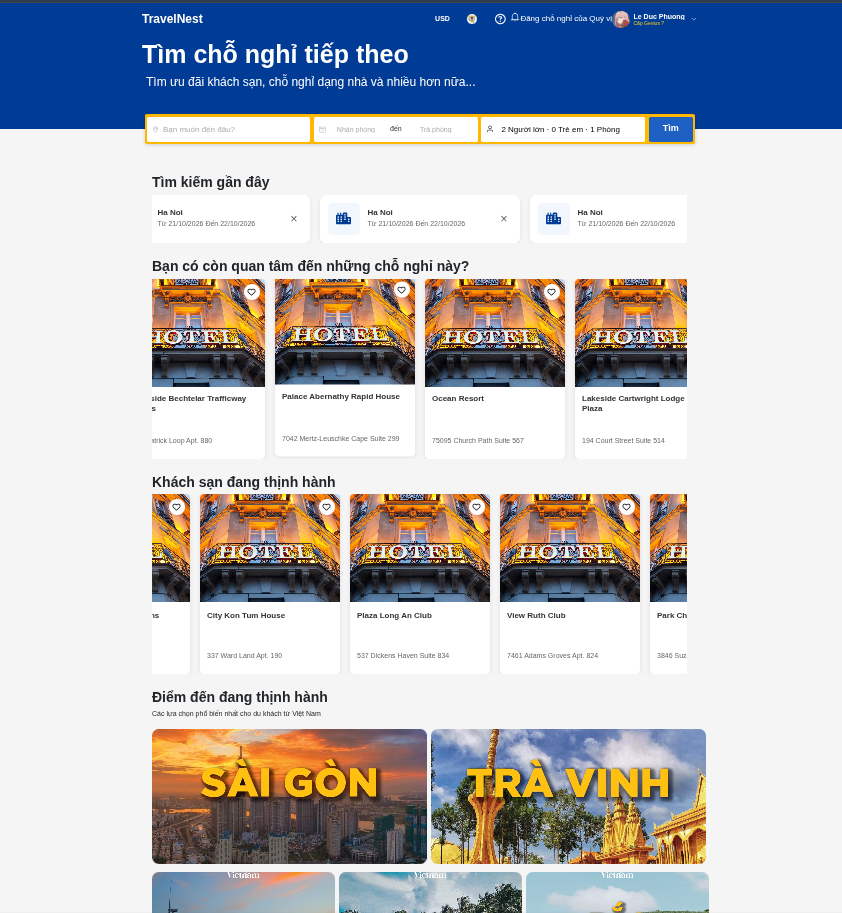
\includegraphics[width=\linewidth]{images/guest_ui.png}
  \end{minipage}\hfill
  \begin{minipage}[b]{0.62\textwidth}
    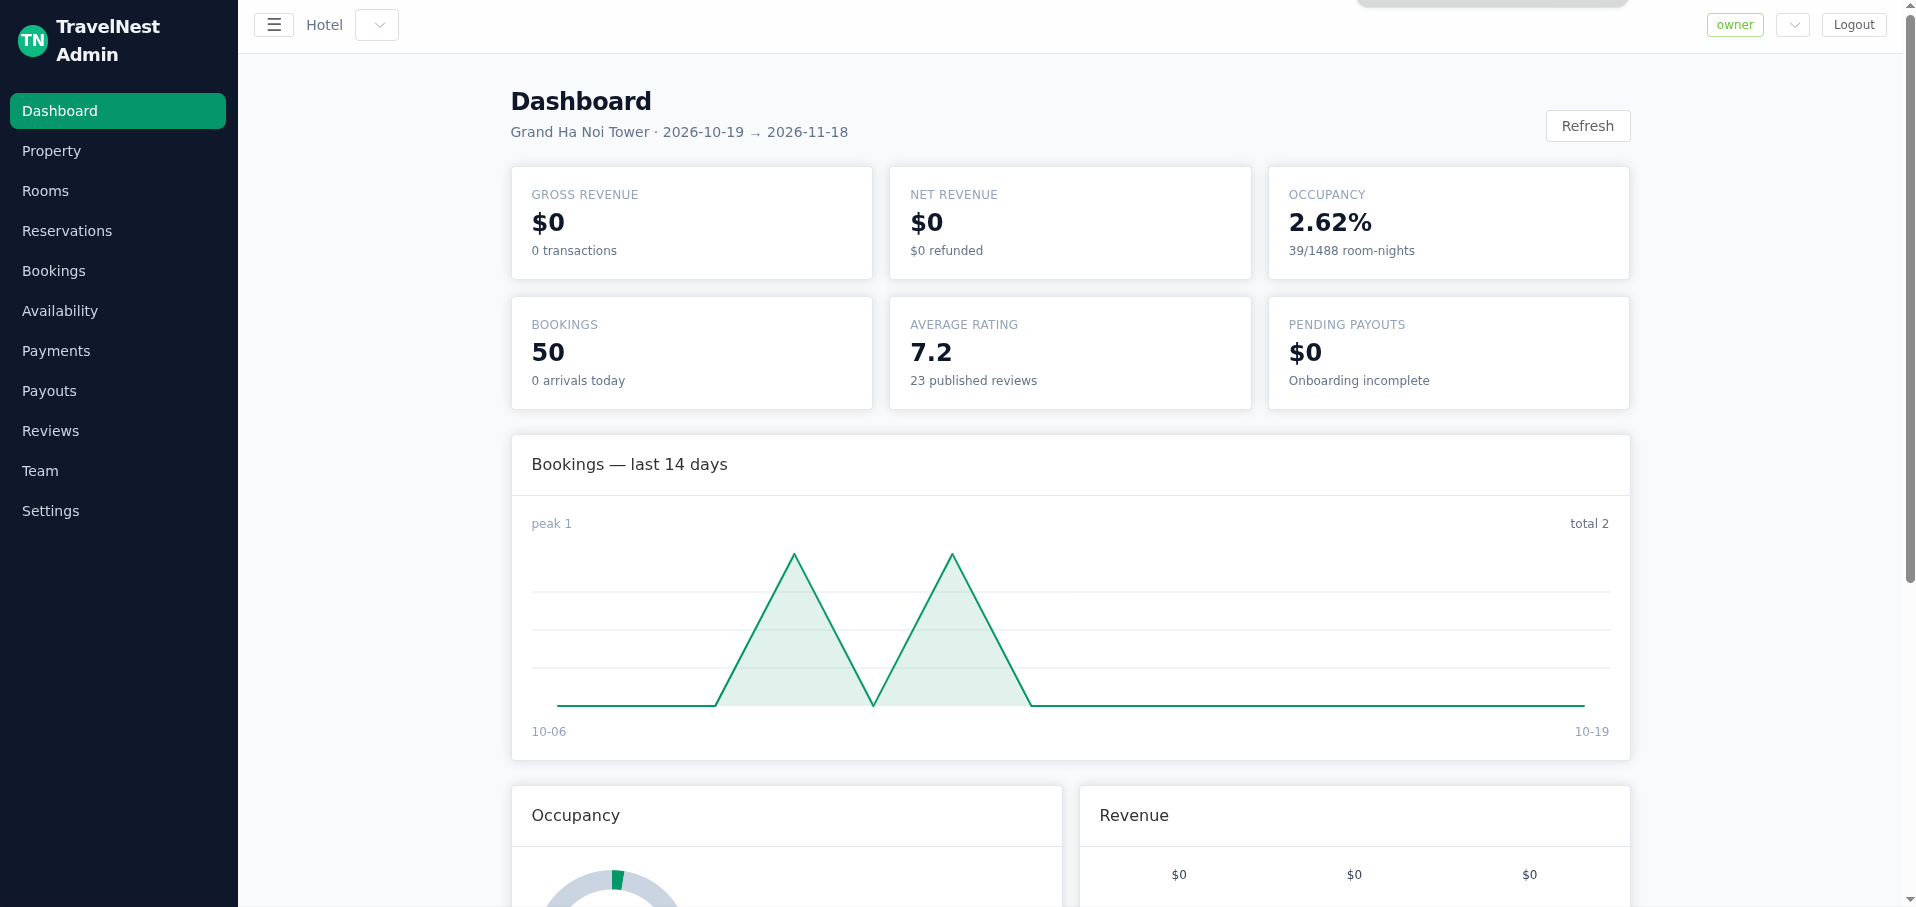
\includegraphics[width=\linewidth]{images/hotel_admin_ui.png}
  \end{minipage}
  \caption{Giao diện khách hàng (trái) và bảng điều khiển chủ khách sạn (phải).}
  \label{fig:ui}
\end{figure}

\begin{figure}[H]
  \centering
  \begin{minipage}[b]{0.48\textwidth}
    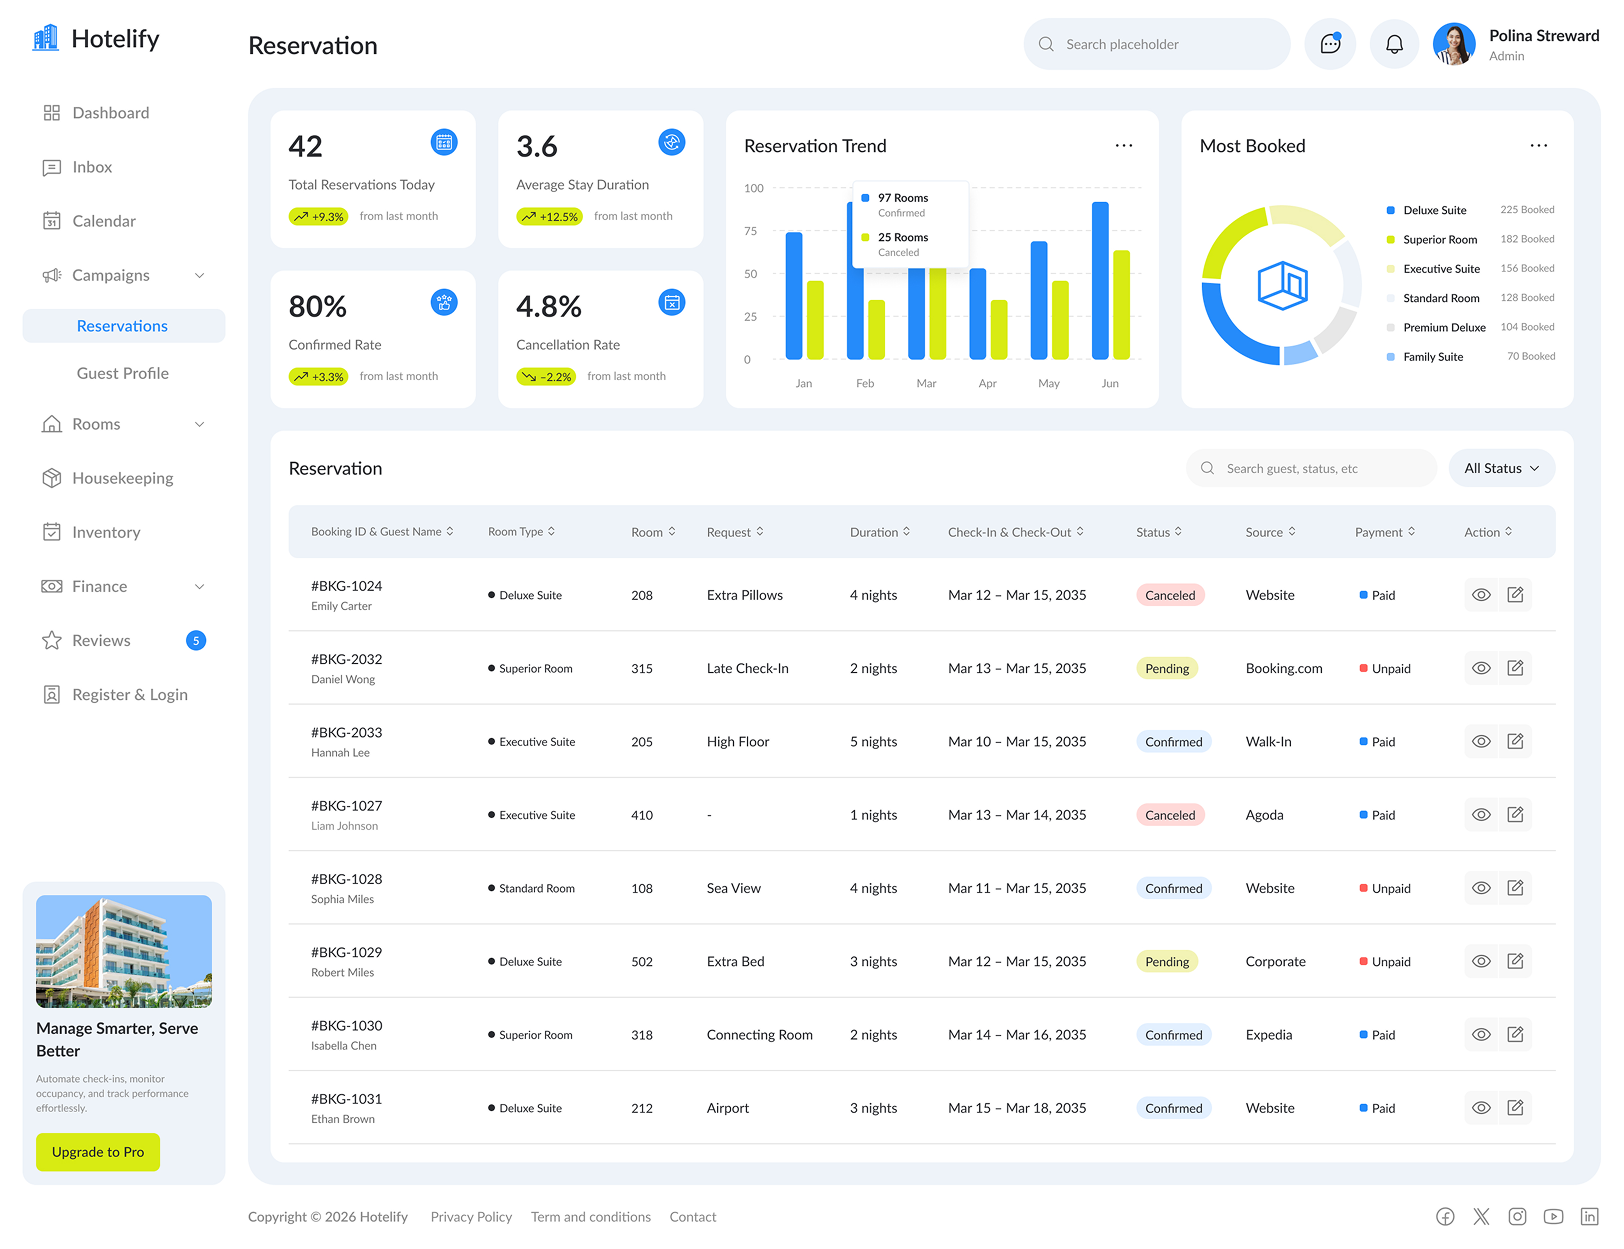
\includegraphics[width=\linewidth]{images/admin_reservation.png}
  \end{minipage}\hfill
  \begin{minipage}[b]{0.48\textwidth}
    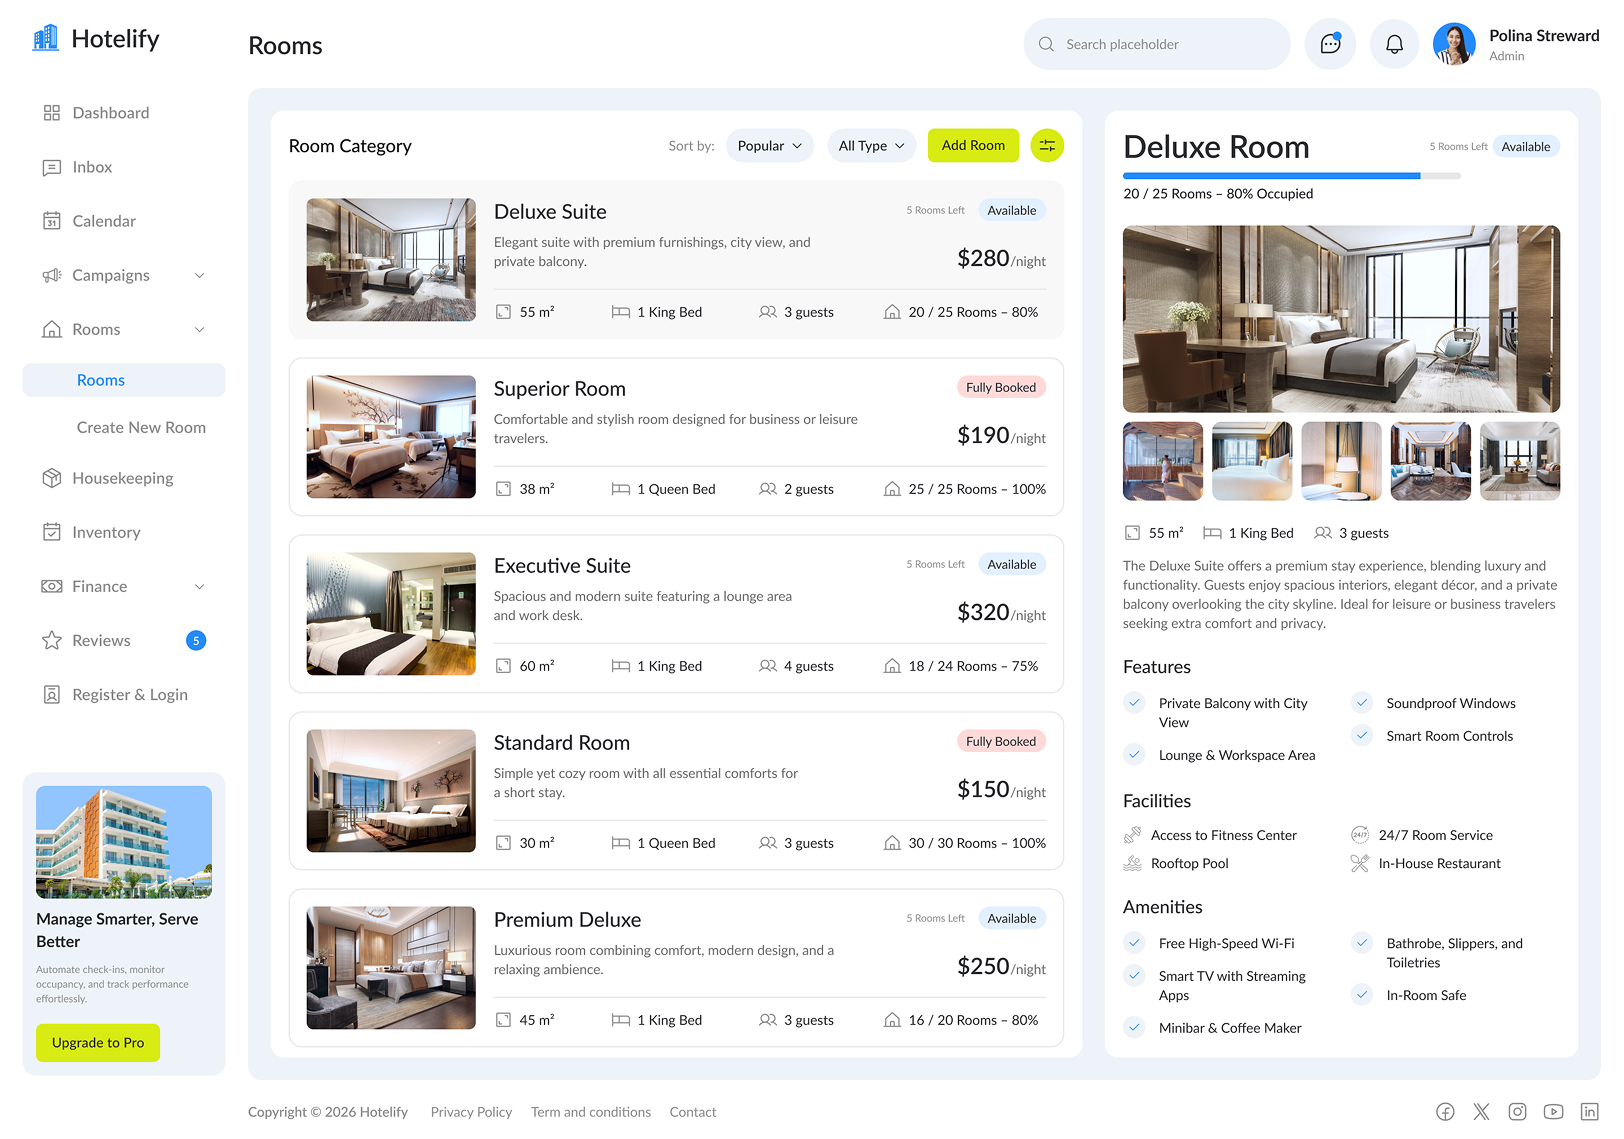
\includegraphics[width=\linewidth]{images/admin_rooms.png}
  \end{minipage}
  \caption{Thiết kế mới (mockup) cho bảng điều khiển admin: quản lý đặt phòng (trái) và quản lý phòng (phải).}
  \label{fig:admin-design}
\end{figure}

\begin{figure}[H]
  \centering
  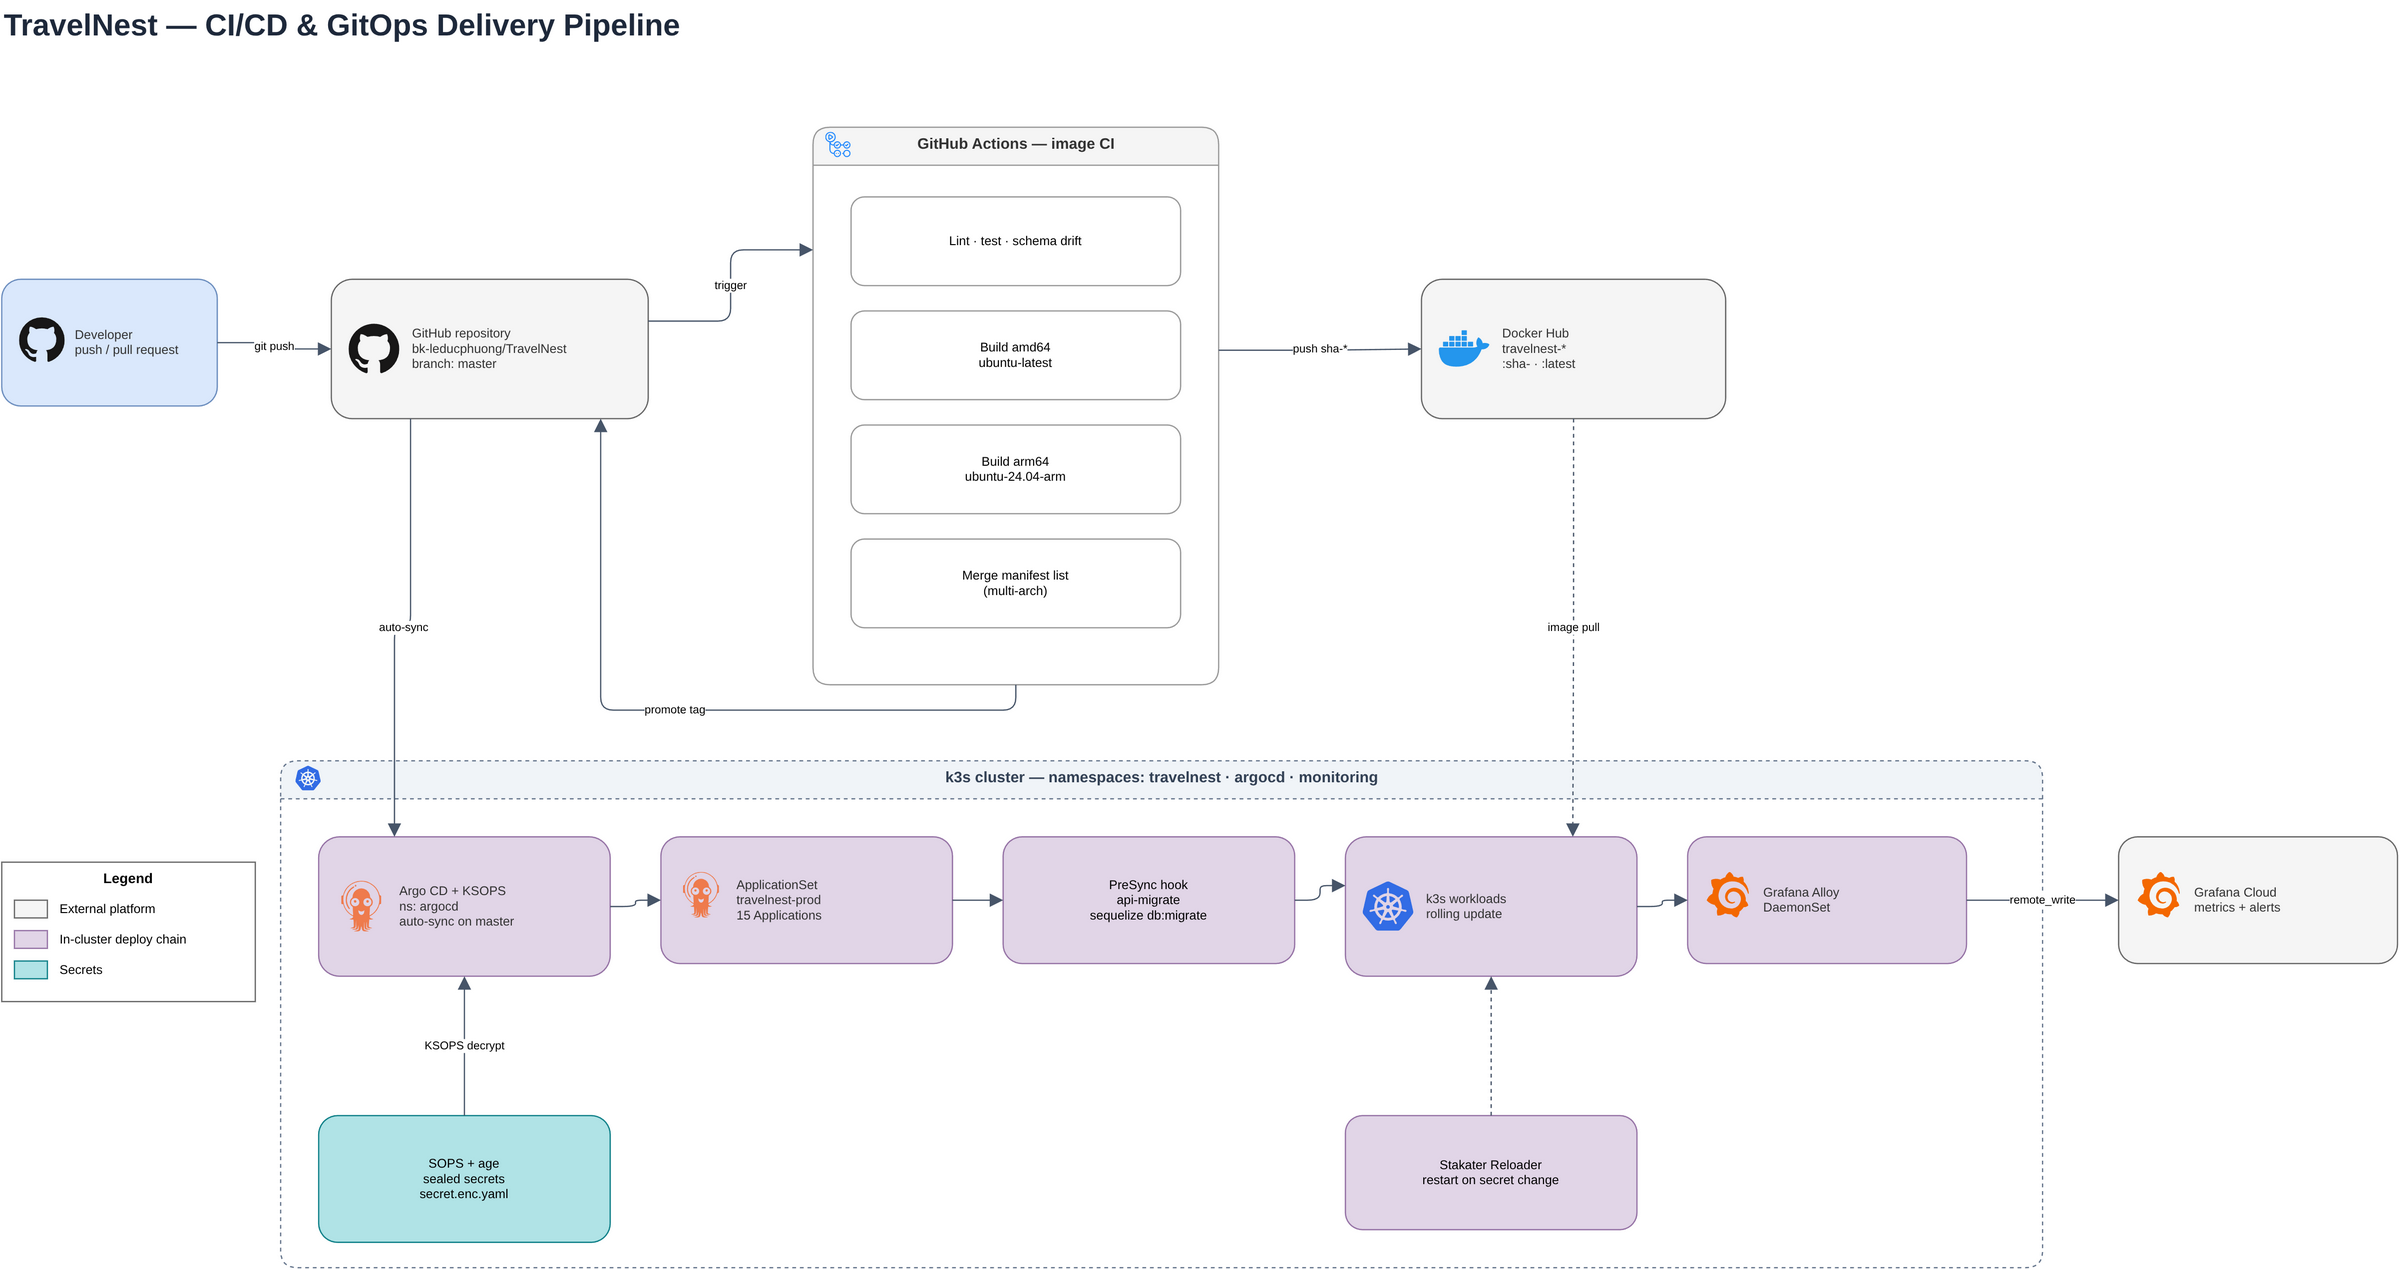
\includegraphics[width=0.88\textwidth]{images/gitops_diagram.png}
  \caption{Sơ đồ CI/CD và GitOps: GitHub Actions build/promote image, Argo CD đồng bộ vào cụm k3s. Bản chỉnh sửa: \link{https://drive.google.com/file/d/1e38Ql1FKK0ohQsn_uKpczDzncas_mthK/view?usp=sharing}{drawio}.}
  \label{fig:gitops}
\end{figure}

\begin{figure}[H]
  \centering
  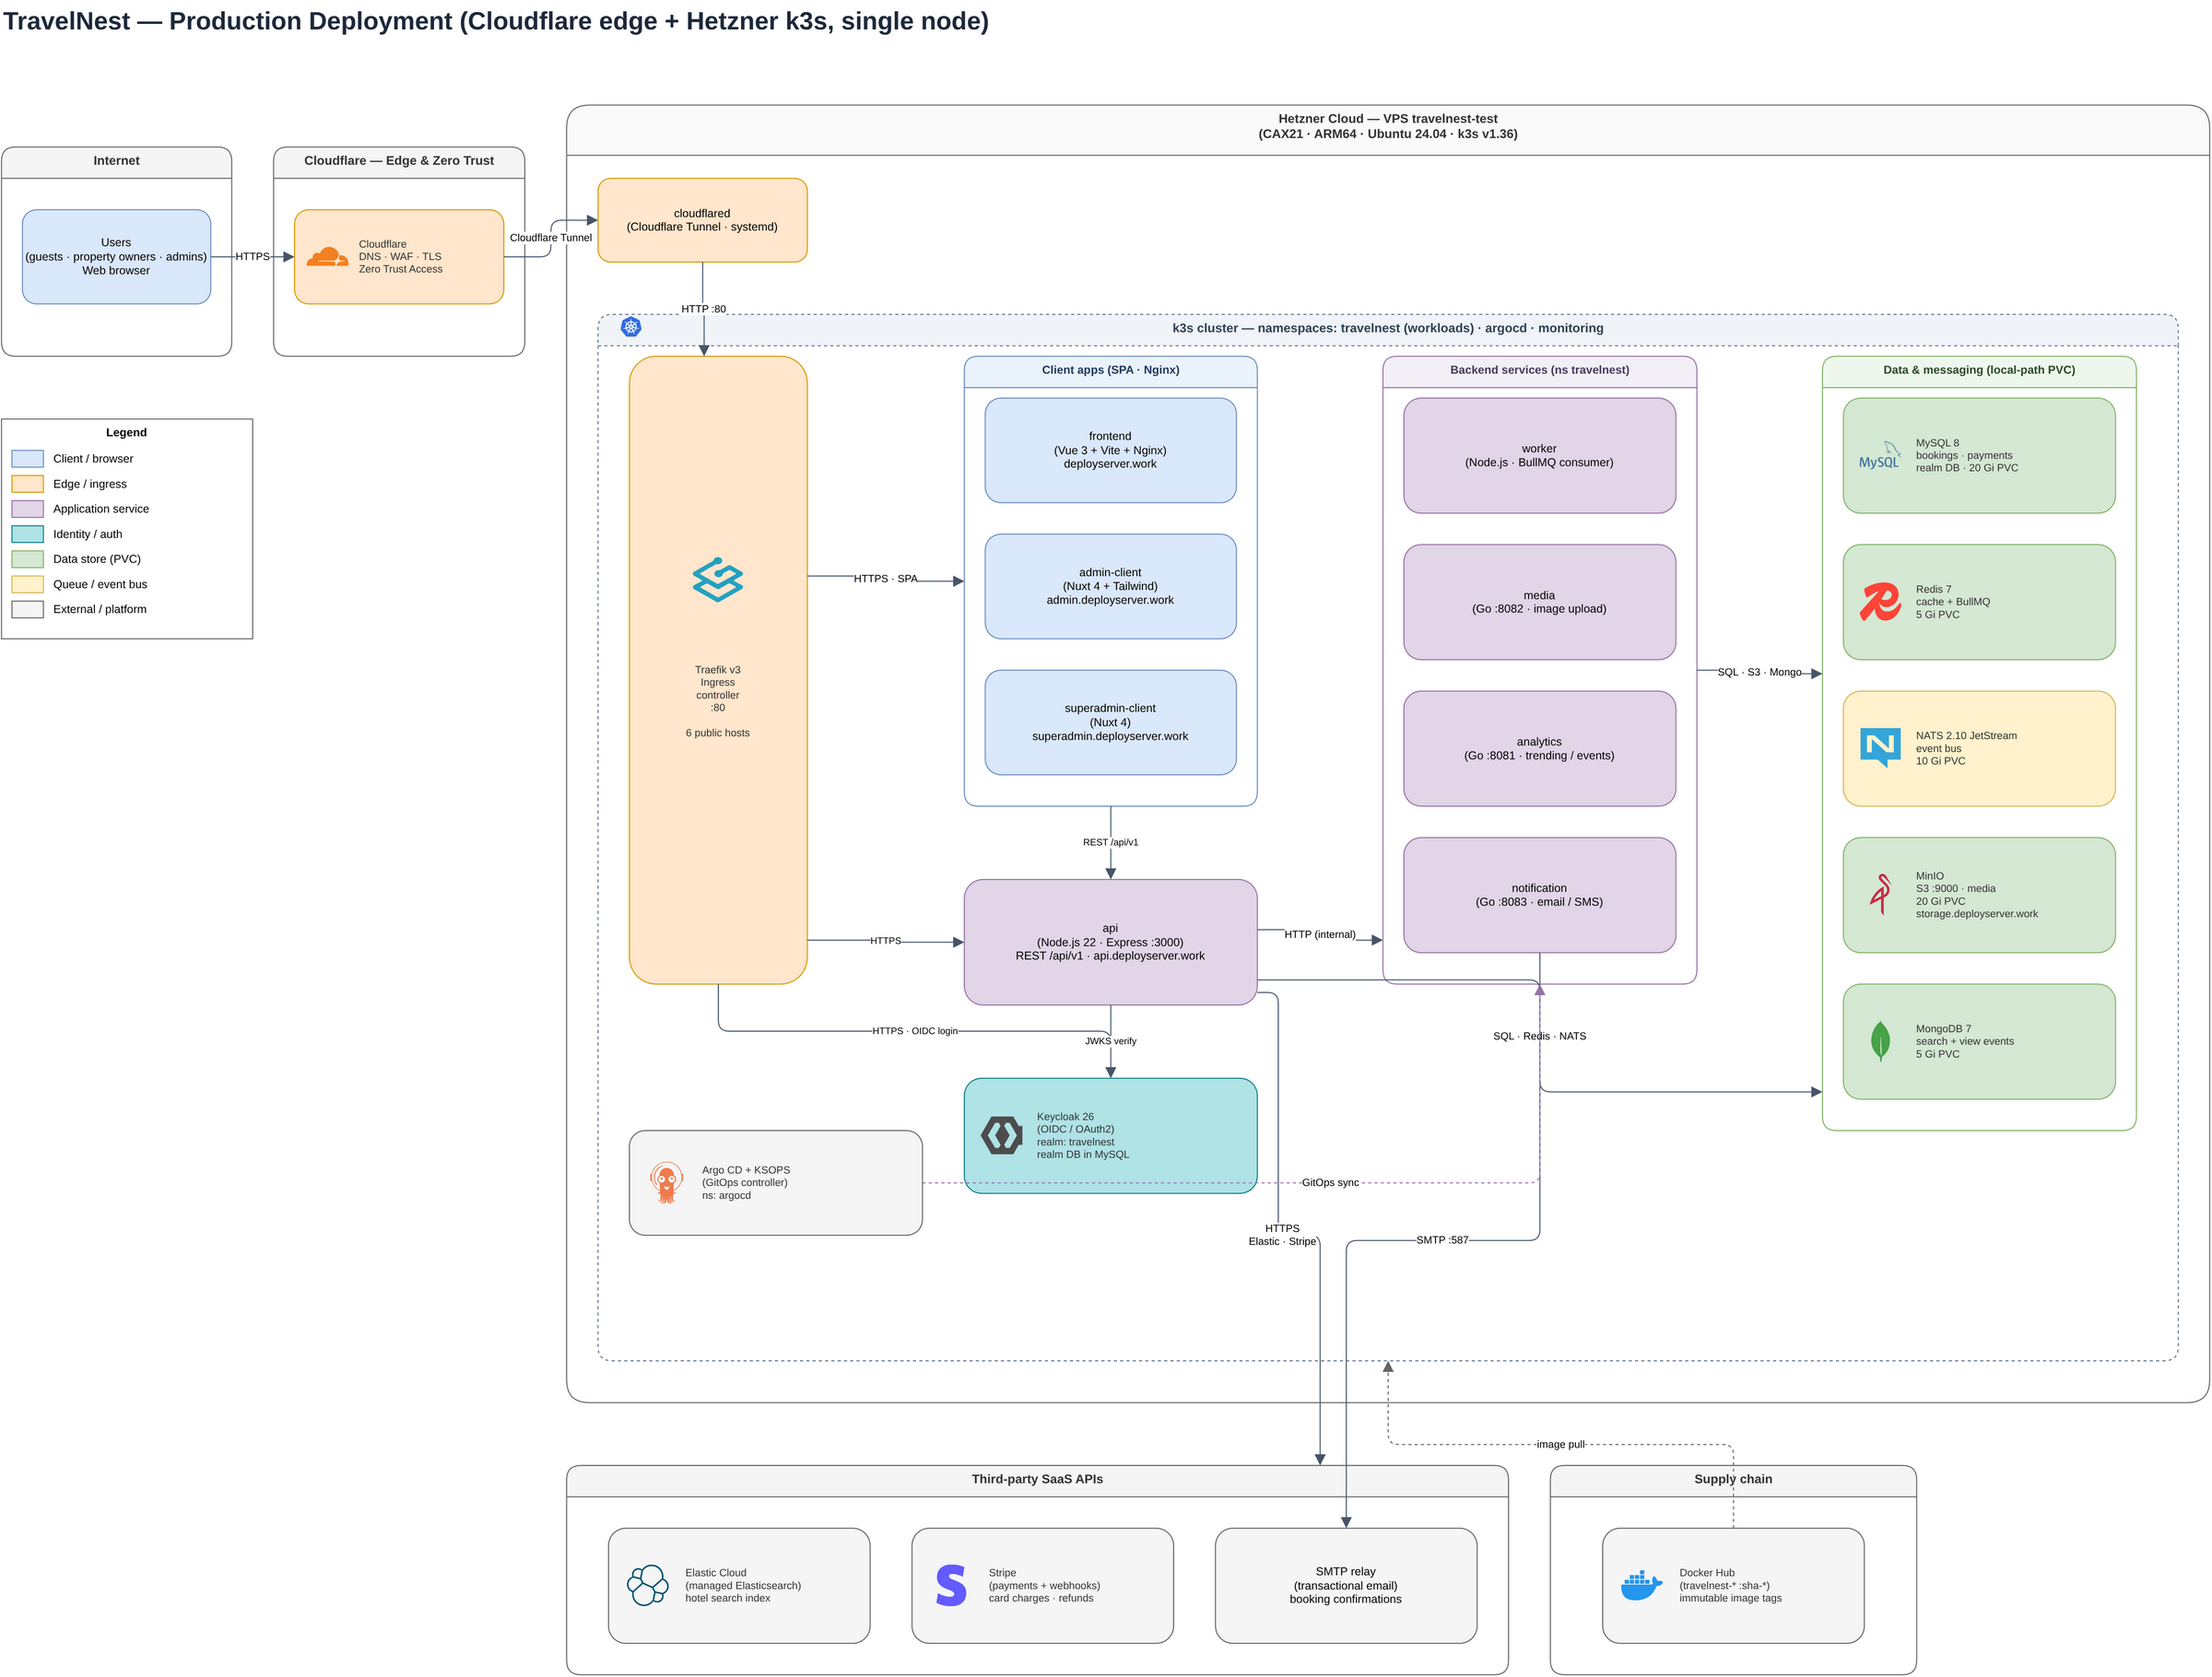
\includegraphics[width=0.82\textwidth]{images/deployment_diagram.png}
  \caption{Sơ đồ triển khai production: Cloudflare Tunnel, k3s trên Hetzner VPS và các dịch vụ/datastore. Bản chỉnh sửa: \link{https://drive.google.com/file/d/19bjapNfXuvRLLnMAehPINVkSJ-ZXZ8DG/view?usp=sharing}{drawio}.}
  \label{fig:deployment}
\end{figure}

\begin{figure}[H]
  \centering
  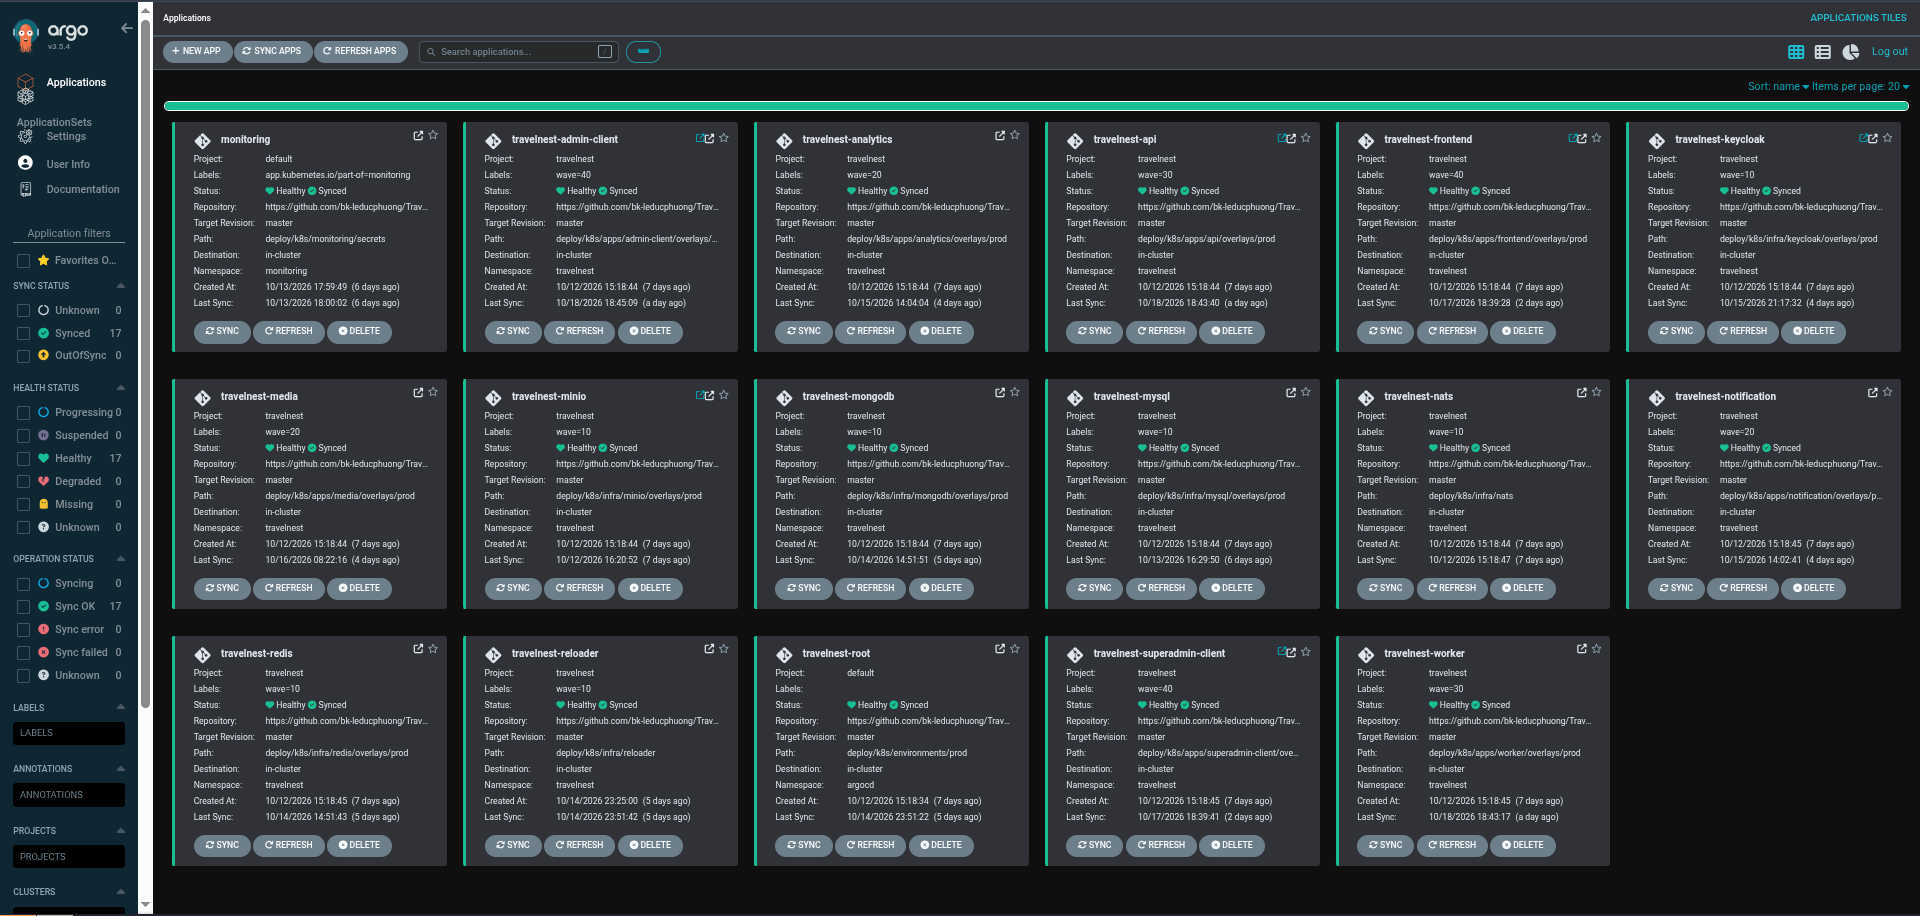
\includegraphics[width=0.88\textwidth]{images/argocd_dashboard_cropped.png}
  \caption{Bảng điều khiển Argo CD: các ứng dụng trong cụm k3s đều ở trạng thái Synced và Healthy.}
  \label{fig:argocd}
\end{figure}

\begin{figure}[H]
  \centering
  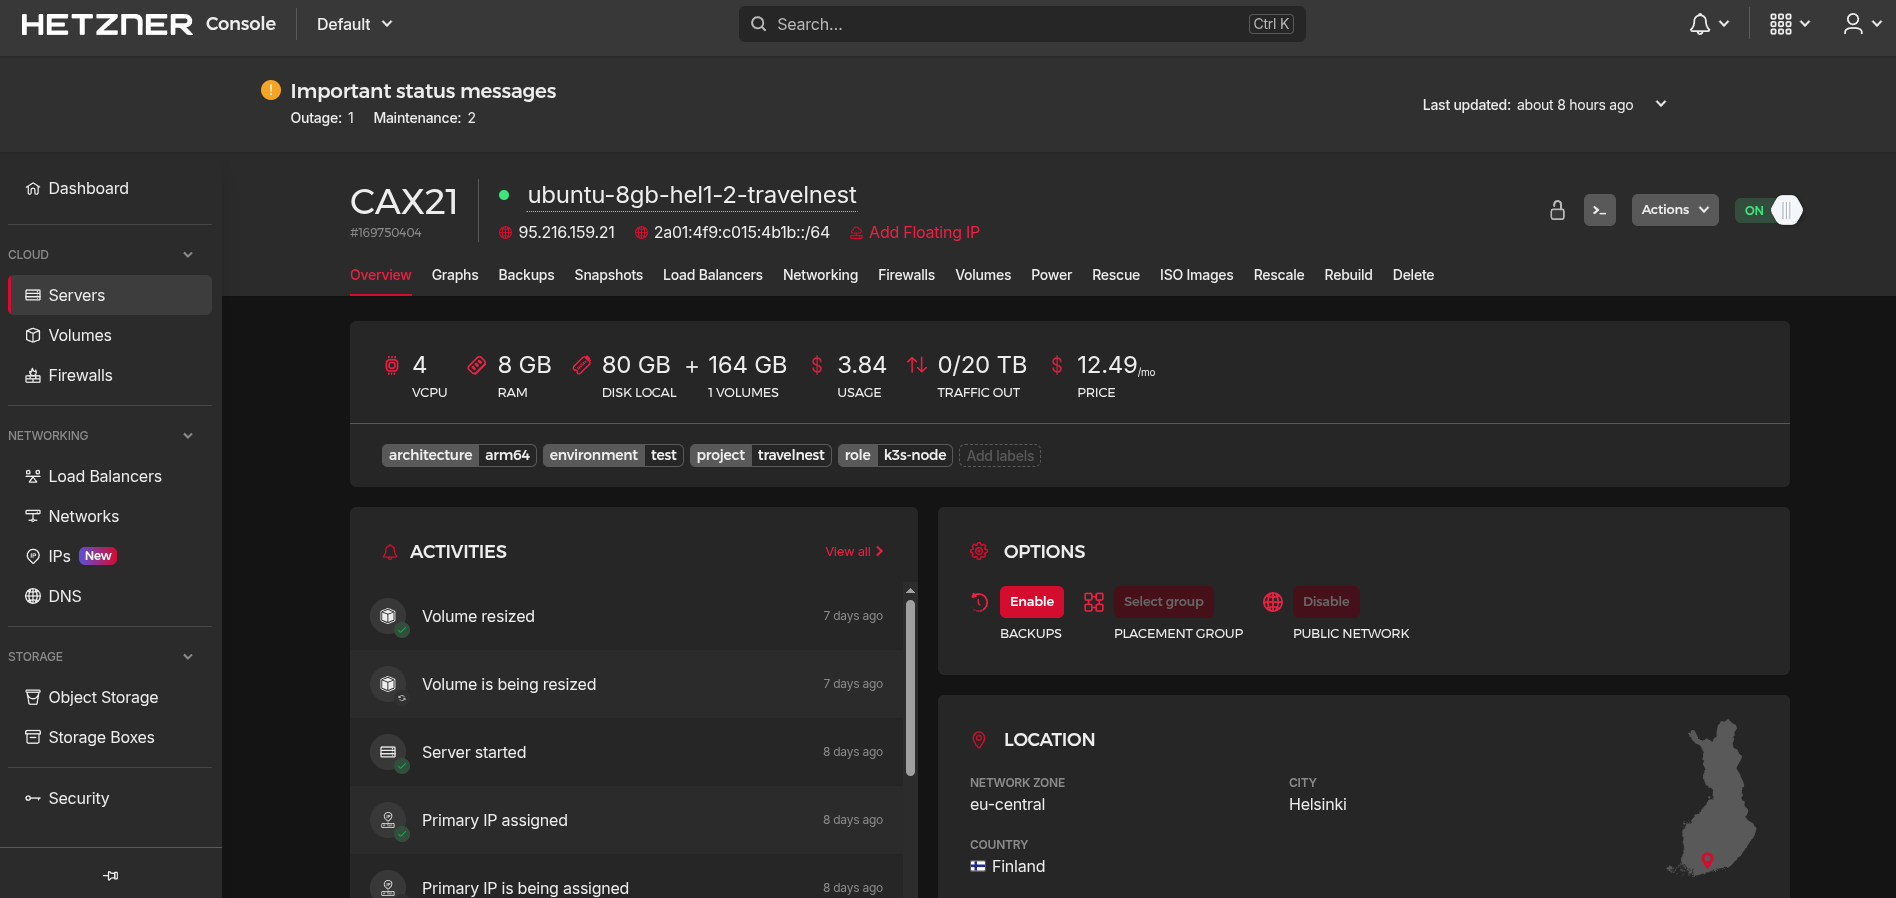
\includegraphics[width=0.88\textwidth]{images/hetzner_dashboard.png}
  \caption{Máy chủ Hetzner CAX21 (ARM64, 4 vCPU, 8 GB RAM) dùng cho cụm k3s.}
  \label{fig:hetzner}
\end{figure}

% ============================================================================
\section{Kết quả đạt được}

\begin{center}
\footnotesize
\begin{tabularx}{\textwidth}{@{}>{\bfseries}p{3.5cm}r>{\bfseries}p{4.1cm}r@{}}
\toprule
Hạng mục & Số liệu & Hạng mục & Số liệu \\
\midrule
Commit / PR & 325 / 46 & Tệp theo dõi & 1.815 \\
Mã nguồn & $\approx$125.000 dòng & Module backend & 13 \\
Dịch vụ Go & 3 & Migration CSDL & 23 \\
Tệp kiểm thử & 147 & Pipeline CI & 9 \\
\bottomrule
\end{tabularx}
\end{center}

\vspace{2pt}
\noindent\textbf{Dữ liệu seed phục vụ kiểm thử.} Dữ liệu demo được tạo tự động bằng pipeline seed (\texttt{yarn demo:seed} cho bộ đầy đủ hoặc \texttt{seed:all:quick} cho bộ rút gọn): xóa dữ liệu cũ, seed lại toàn bộ bảng, upload ảnh trực tiếp lên MinIO, đồng bộ MongoDB/Elasticsearch và provision tài khoản Keycloak. Bộ số liệu tham chiếu dưới đây ứng với cấu hình \texttt{--quick} (63 tỉnh/thành $\times$ 80 khách sạn):

\begin{center}
\footnotesize
\begin{tabularx}{\textwidth}{@{}>{\bfseries}p{2.6cm}X@{}}
\toprule
Nguồn & Dữ liệu theo cấu hình seed \\
\midrule
MySQL & 1 quốc gia, 63 tỉnh/thành, 64 destination, 85 tài khoản; 5.040 khách sạn, 20.230 phòng, 75.653 booking, 50.702 đánh giá, 75.810 ảnh. \\
MinIO & $\approx$151.600 object (ảnh gốc và biến thể WebP). \\
MongoDB & 5.000 search log (90 ngày), $\approx$50.400 hotel view event (30 ngày). \\
Elasticsearch & 5.040 hotel và 64 destination document. \\
Keycloak & 5 tài khoản demo: admin, support, owner, manager, staff. \\
\bottomrule
\end{tabularx}
\end{center}

\noindent Hệ thống chạy công khai tại bốn địa chỉ; mã nguồn: \link{https://github.com/bk-leducphuong/TravelNest-Hotel_Booking_System}{GitHub}, video demo: \link{https://www.youtube.com/watch?v=-jxhmIJp988\&list=PLCt2C1YyUqcCfEhqOXE-Mul8UINudlCse}{YouTube}. Số liệu tổng hợp từ Git đến 17/10/2026; các nhãn trong ngoặc vuông là liên kết có thể bấm.

% ============================================================================
\section{Đánh giá tiến độ}

Ước tính khối lượng hoàn thành của đồ án đến thời điểm hiện tại khoảng \textbf{50\%}. Các chức năng cốt lõi đã chạy được đầu-cuối trên môi trường production; phần còn lại chủ yếu là gia cố chất lượng, kiểm thử và hoàn thiện báo cáo. Minh họa thanh toán: \link{\gh/docs/reports/images/ui_stripe_dashboard.png}{Stripe}.

\begin{center}
\small
\begin{tabularx}{\textwidth}{@{}>{\raggedright\arraybackslash}p{7.0cm}X@{}}
\toprule
\textbf{Hạng mục} & \textbf{Trạng thái} \\
\midrule
Chức năng cốt lõi (tìm kiếm, đặt phòng, thanh toán, quản trị) & Hoàn thành, đã triển khai production \\
Hạ tầng, CI/CD, bảo mật & Nền tảng hoàn thành; còn kiểm thử tải và Stripe live \\
Kiểm thử, tài liệu, báo cáo & Đang thực hiện (phần lớn khối lượng còn lại) \\
\bottomrule
\end{tabularx}
\end{center}

% ============================================================================
\section{Kế hoạch tiếp theo}

\begin{center}
\small
\begin{tabularx}{\textwidth}{@{}>{\raggedright\arraybackslash}p{3.0cm}X@{}}
\toprule
\textbf{Thời gian} & \textbf{Nội dung} \\
\midrule
20/10 -- 02/11 & Hoàn thiện luồng đặt phòng--thanh toán (saga, outbox), xử lý các lỗi còn lại trên guest và admin. \\
03/11 -- 16/11 & Nâng độ phủ kiểm thử, gỡ chế độ cảnh báo khỏi CI, kiểm thử bảo mật và tải. \\
17/11 -- 30/11 & Tối ưu hiệu năng tìm kiếm/ảnh, hoàn thiện monitoring và dữ liệu demo. \\
01/12 -- 21/12 & Viết các chương báo cáo, hoàn thiện hình vẽ và tài liệu tham khảo. \\
22/12 -- 10/01 & Rà soát với giảng viên hướng dẫn, quay video demo và tổng duyệt. \\
01/2027 & Nộp báo cáo và bảo vệ đồ án tốt nghiệp. \\
\bottomrule
\end{tabularx}
\end{center}

\noindent Trọng tâm của phase tiếp theo gồm: hoàn thiện \textbf{refund khi khách hủy booking}, xây dựng \textbf{hệ thống payout cho hotel owner}, và \textbf{cải thiện UI/UX} cho cả guest lẫn hotel admin.

% ============================================================================
\section{Kết luận}

Tính đến 19/10/2026, các mục tiêu chính đã đạt được: TravelNest vận hành đầu-cuối trên production với ba giao diện, backend miền nghiệp vụ và ba dịch vụ Go. Với khoảng 50\% khối lượng, kế hoạch tiếp theo tập trung vào kiểm thử, thanh toán và hoàn thiện báo cáo để bảo vệ vào 01/2027.

\end{document}
